\documentclass[11pt,oneside,a4paper]{article}
\usepackage{graphicx}
\usepackage{booktabs}
\usepackage{caption}
\usepackage{subcaption}
\usepackage{amsmath}
\usepackage{amsfonts}
\usepackage{amssymb}
\usepackage{lscape}
\usepackage{psfrag}
\usepackage[usenames]{color}
\usepackage{bbm}
\usepackage[update]{epstopdf}
\usepackage[bookmarks,pdfstartview=FitH,a4paper,pdfborder={0 0 0}]{hyperref}
\usepackage{verbatim}
\usepackage{listings}
\usepackage{textcomp}
\usepackage{fancyhdr}
\usepackage{multirow}
\usepackage{tikz}
\usepackage{lipsum}
\usepackage{xcolor}
\usepackage[margin=1in]{geometry}
\newcommand{\hint}[1]{{\color{blue} \em #1}}

\makeatletter
\def\cleardoublepage{\clearpage\if@twoside \ifodd\c@page\else%
\hbox{}%
\thispagestyle{empty}%
\clearpage%
\if@twocolumn\hbox{}\clearpage\fi\fi\fi}
\makeatother

\sloppy
% \widowpenalty=10000
% \clubpenalty=10000

\title{
    \vspace*{0.0mm}
    \LARGE\bf\sf Advanced Topics in \\Communication Networks (Fall 2019)
    \vspace*{10.0mm} \\
    \Large\bf\sf Group Project Report \vspace*{30.0mm}\\
    %
    \Huge\bf\sf Hearding the Elephants: Detecting Network-Wide Heavy Hitters with Limited Resources
    %
    \vspace*{30.0mm} \\
    \normalsize
    %
    \sf Authors:\\[5pt]
    \sf Yannick Merkli\\ [5pt]
    \sf Tim Bohren\\ [5pt]
    \sf Felix Rüssli \vspace*{5mm}\\
    %
    \sf  Advisor: Albert Gran Alcoz \vspace*{5mm}\\
    %
    \sf  Supervisor:  Prof. Dr. Laurent Vanbever \vspace*{20.0mm}\\
    %
    \sf Submitted: Dec 16, 2019\\ [5pt]
    \sf \pageref{lastpage} Pages
}
\date{}

\begin{document}

\begin{figure}
    \includegraphics[width=\textwidth]{figures/eth-nsg-header}
\end{figure}

\maketitle
\thispagestyle{empty}
\raggedbottom
\clearpage

\pagenumbering{roman}

\begin{abstract}
Detecting heavy hitters is important for Denial of Service detection, load balancing or traffic routing. We have already seen heavy hitter detection in exercise 4 on a single switch. Protocols in the past always had a trade-off between limitations in communication and memory and accuracy in detecting heavy hitters. Herd however identifies netword-wide heavy hitters in real time, even under bounded communication and memory. The protocol uses probabilistic sampling of flows. The local switches report to a global coordinator. Additionally the coordinator adapts based on spatial locality on the flows.
    %\lipsum[1-3]
\end{abstract}

\clearpage
\setcounter{tocdepth}{2}
\tableofcontents
\clearpage
\pagenumbering{arabic}

\section{Introduction}
\hint{Introduction to the problem that was solved in this project.} \\
Heavy hitters are flows that are responsible for a large number of packets inside a networks. Networks operators are interested in spotting them in order to prevent Denial of Service attacks or maximes the sending rate. Heavy hitters can also be used for network management such as usage-based pricing or load balancing. To effectively protect networks from attacks network operators need to detect heavy-hitters quickly. 

Since the operators only have limited resources, especially when it comes to memory and processing power, they have to choose between good accuracy and small delay.

Further heavy hitters don't necessarily need to come towards a single ingress switch. They can also be incoming from a dristibuted source and thus as a mix of smaller flows over multiple ingress switches, which add up to a heavy-hitter. %(DDoS?)

%very small description of Herd
Herd solves these problems by sampling traffic, which saves memory on the switches, and reporting to a global coordinator once the observed flows grow larger in size, and thus still keep good accuracy in detecting heavy hitters. The coordinator looks at flows from all over the network. Therefore Herd enables us to add medium-sized flows together from all over the network. This system makes it possible to not only detect local heavy hitter, but also distributed ones, potentially even detecting distributed Denial of Service attacks, before they grow to their full potential.

%\lipsum[1-2]

\section{Background and related work}
\hint{Briefly describe background information and related papers (if any). You do not need to describe topics that were coverd in the lecture, only other topics that are relevant for your project.} \\
Heavy hitters are flows that are responsible for a large number of packets inside a networks. Networks operators are interested in spotting them in order to prevent Denial of Service attacks or maximes the sending rate. Heavy hitters can also be used for network management such as usage-based pricing or load balancing.

Since heavy hitters are so large they are often called elephant flows, in contrast to the small and numerous flows, which are called mice. There already exist a number of protocols with multiple different approaches to spot these elephants. One idea is to sample the incoming traffic, for example NetFlow\cite{claise2004netflow} or the sample-and-hold protocol\cite{estan2003sample}. Other approaches use sketches, e.g. the count-min sketch\cite{cormode2003countmin}, or bloom filters, such using the counting bloom filter we used in exercise 4. MG-algorithm\cite{mg1982repeat} and the EARDet\cite{wu2014eardet} on the other hand use a streaming based procedure. 
However all these protocols suffer from a trade-off between accuracy and efficiency.

We take here a closer at the sample-and-hold algorithm\cite{estan2003sample} since it has an important role in Herd.

Incoming packets first get checked whether their flow is being kept track off. If it is, we increase a counter value associated with it.

If the according flow is not being monitored, e.g. since it is the first packet of that flow, the switch starts keeping a record of it with
a probability $s$.\\

samplecitation:\cite{bosshart2014p4}
%\lipsum[1-2]


\section{Implementation}
\hint{Describe how you solved the problem and how your implementation works. Do not paste source code here.} \\
Herd uses local ingress switches and a central coordinator to get a global view. Further Herd categories the flows of packets into four different types: mice, moles, mules and elephants.

\subsection{From mice to elephants} \label{animals}

\begin{figure}
	\centering
	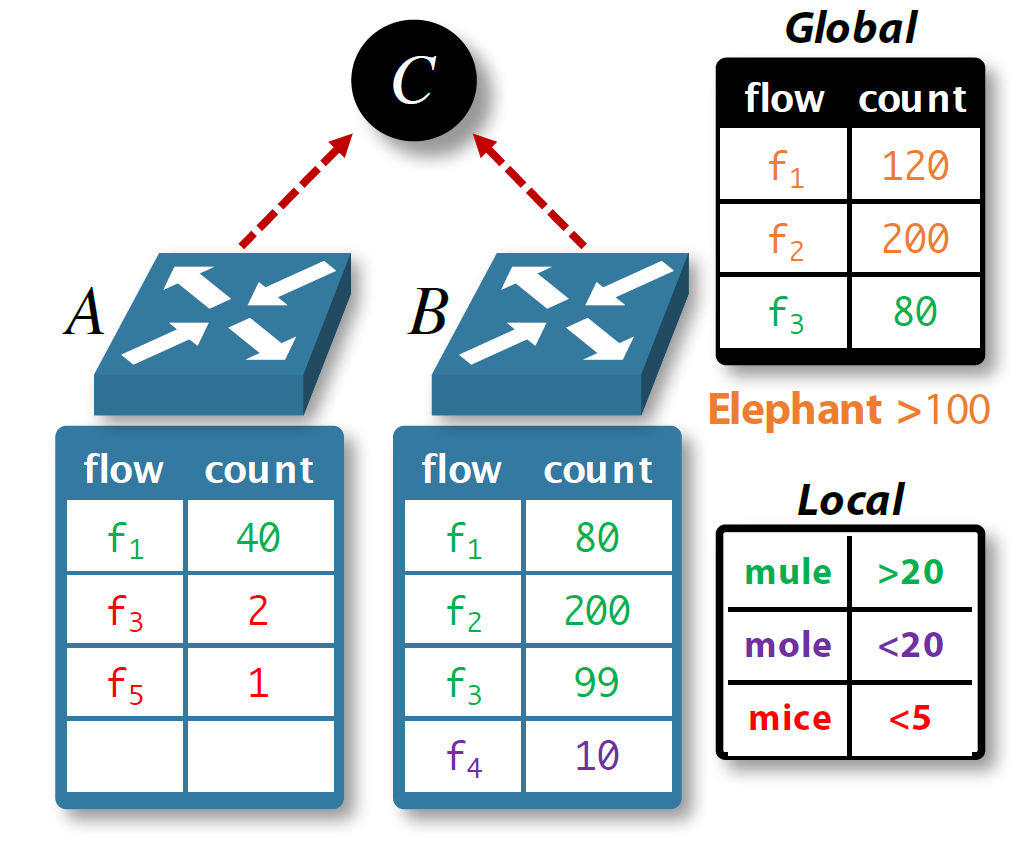
\includegraphics[width=0.5\textwidth, scale=1]{figures/paper_zoo}
	\caption{Zoology in the Herd protocol. \cite{anon2019herd}}
	\label{fig:zoo_fig}
\end{figure}

All flows start as mice. Mice are most numerous but also the smallest flow type. When a packet arrives Herd uses the sample-and-hold algorithm descibed above to remember some of the flows since the switches only have limited. With an increasing number of packets of a flow arriving on the switch the more likely the algorithm memorizes that flow.

Once a flow is captured by an ingress switch it advances to the next higher tier: the mole. A mole simply a flow on which a local switch keeps track of the number of packets it observers.

Each time a mole flow is observed $\tau$ times by the local ingress switch it tries to report this flow to the global coordinator switch with the probability $r$. Flows are only announced to the coordinator once they are seen $\tau$ times for two reasons: First, the global coordinator should also not waste it precious memory on every mouse flow that happens to be caught by the switch. If instead the Herd switch ensures that the flow is used $\tau$ times the flow has the potential that it could grow to a heavy hitter, especially when the reports of other ingress switches are taken into account. The other reason is, that the network does not have infinite bandwith, so the switch has to be careful to not clog up the link with reports to the coordinator. For that reason the switch does not send a report each time is has seen $\tau$ packets but only with the probability $r$. The flows that arrive at the coordinator are now mules.

The coordinator has a global view of all the mules from the ingress switches which have Herd running on them. In contrast, the ingress switches only have a local view since they do not know what the other switches observe. The coordinator counts how many reports of a flow are sent to it, independent from which ingress switch it arrives from. As soon as the coordinator has seen at least $R$ reports of a flow is classifies that flow as elephant, which is how heavy hitters are called in our small animal kingdom.

\subsection{Locality} \label{locality}
So far it was assumed that all ingress switches have the same probability to observe a flow. However in real networks flows often cross switches based on locality between them. So, different switches are more likely to observe different flows. This concept has an effect on the size of $\tau$. The fewer ingress switches see a flow, the higher $\tau$ is, since it is unlikely that an unrelated switch comes across this flow. Out of this follows that ingress switches are less likely to promote a mole to a mule which is not even a global elephant. %This part is a bit wonky...

Herd tracks the locality $l_f$ of a flow $f$ dynamically. If the ingress switch encounters a unexpected flow $f$ it sends a message to the coordinator. The coordinator then updates internally which switches see the flow $f$ and reports back to the switch with $l_f$. Of course the coordinator also has to inform the other switches which observe $f$, but it only does that once the number of observing switching has doubled to save on bandwidth.

Now, storing an $l_f$, $\tau_f$ and $r_f$ for every five tuple $(srcIP, dstIP, srcPort, dstPort, protocol)$ on the switches uses too much memory. Thus, Herd keeps track of the locality based on groups. These groupes are only depending on the two tuple $(srcIP, dstIP)$.

\subsection{Tuning the parameters} \label{tuningparameters}
Until now it was assumed that the parameters $\tau$, $s$, $r$ and $R$ were given. Now we try to find those paramaters in order to maximize the detection accuracy of Herd under communication and switch memory constraints. We do this by simulating the whole protocol for one Herd switch and the coordinator. In tuningparameters.py one can specify the packets needed to promote a flow into a heavy hitter and a set of training data in form of a pcap-file, but also the limited switch memory and communication budget. The program then iterates through the possible approximation factors $\epsilon$ and returns the parameters which maxime the accuracy.

First, we try to configure the sampling probability $s$ of the sample-and-hold algorithm. With unlimited switch memory $S$ the sampling probability could simply be set to $s=1$ and the switches would memorize all flows going through them. Let $M$ be the set of observed moles on the switch. Thus the switch has to store $|M|$ different flows. From this we conclude that we need $|M| \leq S$ in order to be able to store all the observed flows. To be sure that the real $M$ has enough space in $S$ we even want $|M| < S$. In order to have this in expectation $s$ is set to $1/\tau$. For that an estimation of $\tau$ is needed. At the beginning $\tau$ is set to the global threshold $T$. $T$ is the size a flow needs to have in order to be recognized as a heavy hitter. Then we look in our training data $D$ how many moles are found and check whether the found moles $M$ use up all the memory $S$. Afterwards $\tau$ is made smaller to increase the chance to categorize a flow as mole. This is done iteratively as long as there is still space in $S$. 

If unlimited bandwidth was available $r$ could be set to 1, since there would be more than enough bandwidth to send all the mule reports to the global coordinator. Further, the coordinator would need at least $R = T/\tau$ reports to classify a flow as elephant. However, under the communication budget $C$ the parameters $r$, aswell as $\tau$ and $R$ need to be adjusted. This is done with the help of the approximation factor $\epsilon$. We approximate global threshold with $\epsilon$ and expect to see at least $\tau$ packets of that flow on every local switch with that flow, so in $l$ switches. This brings us to the equality $\tau l = \epsilon T$, from which we get $\tau =$ $\epsilon T\over l$. Now that we have again a $\tau$. We calculate now first the set of moles $M$ from our training data, and then from that the set of mules $U$ since the necessary $\tau$ is now available for that. The total number of sent reports can be bound with $T|U|r\over \tau$ which leads to $r =$ $T|U|C\over \tau$. The coordinator needs to see at least $R =$ $lr\over T$ reports. We can now finally adjust $\epsilon$ in steps of $\sigma =$ $l\over T$ since $\tau$ is an integer. Everytime we change the value of $\tau$ we calculate $\tau$, $r$ and $R$ anew aswell. This is done until the accuracy decreases for the first time. Afterwards the program returns the optimal parameters and terminates.

\subsection{Switch logic} \label{switch}
Herd uses randomness for sampling packets and reporting to the global coordinator. Of course p4 doens't have a random library. Therefore hashes are used to 'flip' coins and simulate randomness. Further the switch can't process floating point numbers. For this reason the coordinator converts the probabilities into 32-bit numbers. In the flip action this numbers are then compared to hashes. Depending on the comparison a flip-flag, which represents a True or False, is either set or reset. This flag represents whether the random coin toss was successful or not.

A packet arrives at the switch. The switch extracts the first 8 bits to look up the group value of the packet. For unknown groups the switch sends a hello message to the coordinator, which reports back to the controller with a locality parameter for the group. For known groups the switch uses tcpthe sample-and-hold algorithm to either make a new entry in one of the three hash tables or increase the value associated with the flow. If the local thresh $\tau$ was reached flip again a coin. If the flip was successful tell local controller to report to coordinator and reset the counting value. 

\subsection{Controllers} \label{controller}

\begin{figure}
	\centering
	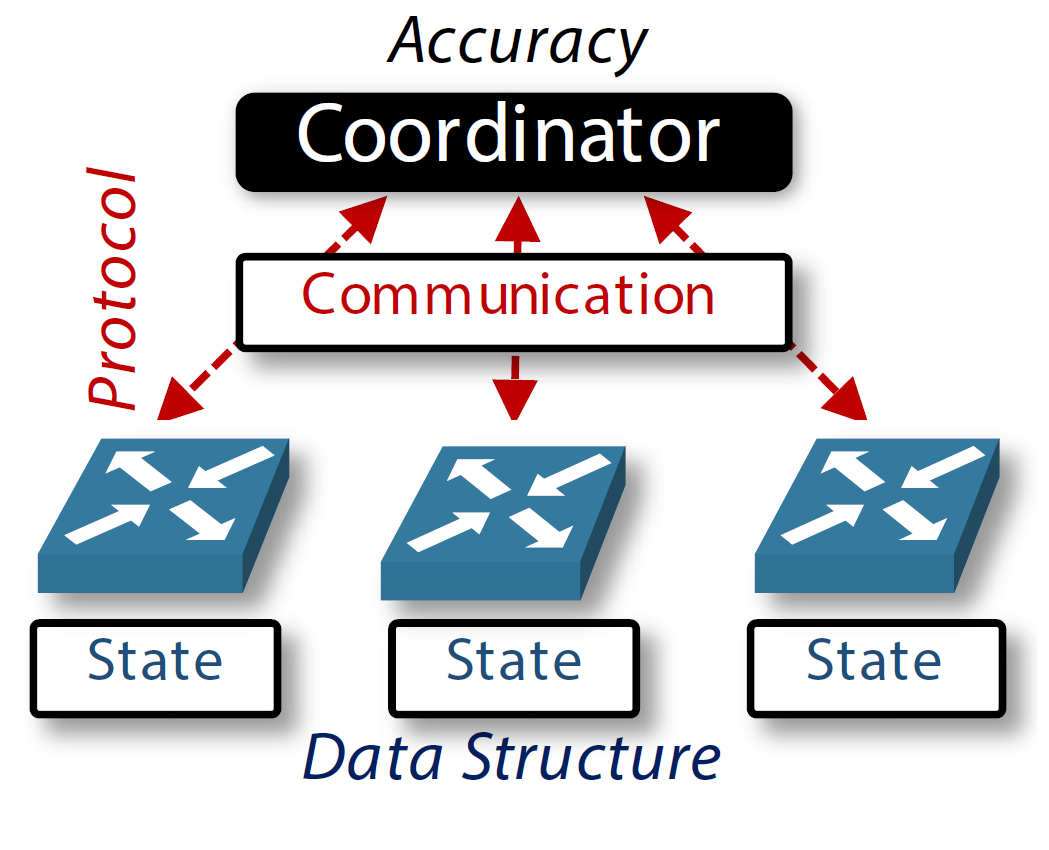
\includegraphics[width=0.5\textwidth,scale=1]{figures/global_local_paper}
	\caption{The Herd switches communicate with the coordinator. \cite{anon2019herd}}
	\label{fig:global_fig}
\end{figure}

When writing 'controller' in this section the L2Controllers are meant, so not including the controller of the coordinator. 

The L2Controller starts by cleaning all the hash tables. Then it fills in the forwarding table. In our testing setup the switches with Herd on them only have two neighbors, a switch for load balancing between the ten Herd switches and an aggregating switch which sends traffic to the end hosts.

Further, the controller runs a digest loop in order to handle the communication between the data and the control plane of the programmable switch. The controller unpacks the received digest message. For each flow the controller checks whether it has seen that flow before. If the flow was not seen before the controller sends a hello to the coordinator, but only if this wasn't already done for the group of the flow. The group is simply a two-tuple consisting of the source- and the destination-IP. When sending a hello the controller expects a callback from the coordinator, telling it the according locality parameter. The coordinator can then calculate the according group parameters $\tau_g$ and $r_g$. If it is a known flow the controller sends a report. %"digest loop"

\subsection{Coordinator} \label{coordinator}
The global coordinator handles all the messages sent to it and reports back with new locality parameters to the individual switches if necessary. 

When a hello arrives from a switch the coordinator checks whether the coordinator has already seen the switch or the flow before. If not it saves them. Now the coordinator uses the HandleHello function from the original paper. First it checks whether it had already got a hello from that switch with that flow. If not if saves it in the dictionary $S_f$ and finally sends notices all switches in updated $S_f$, but only if the size of $S_f$ doubled in order not to overwhelm the links with update messages. If $S_f$ didn't double in size, the coordinator only sends a notification to the new switch in $S_f$ about the current size of $S_f$.

Handling the reports is quite simpler. The coordinator simply counts the number of reports arriving at it for each flow. And after enough reports arrived the flow get put into a list with all the other heavy hitters. Finally upon shutdown it writes found elephants into a $.json$ file for further processing.

\subsection{Additional expansions} \label{special}%title
%problem explanation, see below
If all three hash tables storing the counter values to the flows on a switch were to be full this switch couldn't handle new flows anymore. Therefore in that case the switch informs the controller with a error message. The controller subsequently resets the hash tables. 

\subsection{Challenges} \label{challenges}
Since the traffic we received from CAIDA for the evaluation had no MAC addresses we had to append our own created MAC addresses. 

The topology for the evaluation needs an additional load-balancer in front of the switches running Herd. This is needed in order to distribute the packets across all the ingress switches from $h1$. 

Additionally the load-balancer has to distribute the flows randomly between two randomly chosen switches. 

At the other end of the ingress switches we had a similar problem. This is why we put an aggregating switch between the ingress switches and $h2$. This switch collects again all the packets from the ingress switches and forwards them to $h2$. 

We faced further challenges with the communication between the ingress switch controllers and the coordinator. Since the communication between those two is asynchronous, for example a report about a mule could arrive at the coordinator before the hello and therefore not be store.%uh... really? I think the example is wrong.

The original paper mentions the implementation of a rolling window which resets the hash tables every $W$ seconds. Further, once all the hash tables are filled the ingress switches were to send every single sampled packet of a new flow to the global coordinator. So basically these new flows would have $\tau = 1$ and $r = 1$. The coordinator would therefore pretty much instantly classify these flows as heavy hitters even if they aren't. We didn't like this solution of the rolling time window since it doesn't solve the problem of what happens to new flows once the hash tables are full. We solved this problem by instantly resetting the hash tables once they can't accomodate a new flow, and therefore not waiting until the window $W$ is closed. Our solution doesn't overflow the coordinator with reports about the new flows.

Further we faced severe speed issues. The scapy library often reached its limit in terms of speed. Another challenge was that the pcap files are often so big that it takes a long time to test the implementation of Herd. This makes the testing process even slower together with scapy. 
%how we solved it. I need to have explained again.

We ended up using copy-to-CPU in trying to increase the speed. Further, tcpreplay is used in order to send packets specified in the pcap file from the host $h1$. We also recompiled the p4app without logging and debugging disabled. However, all this didn't help much. Already with not much more than 200 packets per seconds many packets didn't make it to the coordinator. We suspect that during the time coordinator needs to process a hello the ingress switch somehow loses lots a packets.

However, the speed issues we faced are only a problem in software, since the speed of the whole architecture in would be a multiple of the speed in software when implented onto hardware.

\subsection{Assessement of the original paper} \label{original_paper}
Due to the original paper on being only a rejected conference submission and not an accepted paper we faced many challenges along the way. The authors are often vague. For instance the topology used for evaluation is barely mentioned. The paper also contains mistakes. For example in the GetSampling function the sampling probability is not adjusted in the while-loop which could trap the program in an infinite loop. The idea of a rolling time windows sounds rushed. This is why we implemented that the switch resets once the table is full.

Many import ideas of the protocol and its assessment are only mentioned with a few words, or not even all. The unit of the communication budget $C$ can only be guessed since it is written once on a graph, the unit of the state constraint $S$ is never mentioned at all. Even though large parts of the algorithm for the tuning of the parameters is in pseudocode many section are unclear and substandartly explained. Section 5.2 of the paper is especially poorly explained. Even though it explains the algorithm "DeriveReporting" the formluas are barely derived at all. %too harsh?
Many key ideas are not explained at all, for example where to data set for the tuning algorithm is derived from or from where the algorithm knows the number of switches which observe a flow $l$, Since algorithm doesn't seem to be embedded into the running protocol. The authors seem to solve this problem by using a constand $l$ of 2 in their evaluation.

What happens when all the hash tables are full is mentioned in a single cryptic sentence. Luckily, we were able to solve this issue ourselves by emptying the tables in such an event.

The whole evaluation section is a mess.%Maybe a bit harsh.
The figure 6 (a) and (b) don't say much at all since it only measures the precision. Precision only takes false and true positives into account,  but false negatives, which very import for a heavy hitter detector, are completely omitted. Again the lack of overall units makes the understanding of the graphs unnecessary difficult. The Tuning Efficacy is not a bad idea per se, but the last paragraph of the evaluation is very unprecisely written. The two graphs belonging to that section seem very rushed, they don't even have the measured parameters attached to the axis and the heat meter.

%\lipsum[1-5]

\section{Evaluation}
\hint{Describe how you tested your implementation and summarize the results.} \\
\subsection{Topology} \label{topology}

\begin{figure}
	\centering
	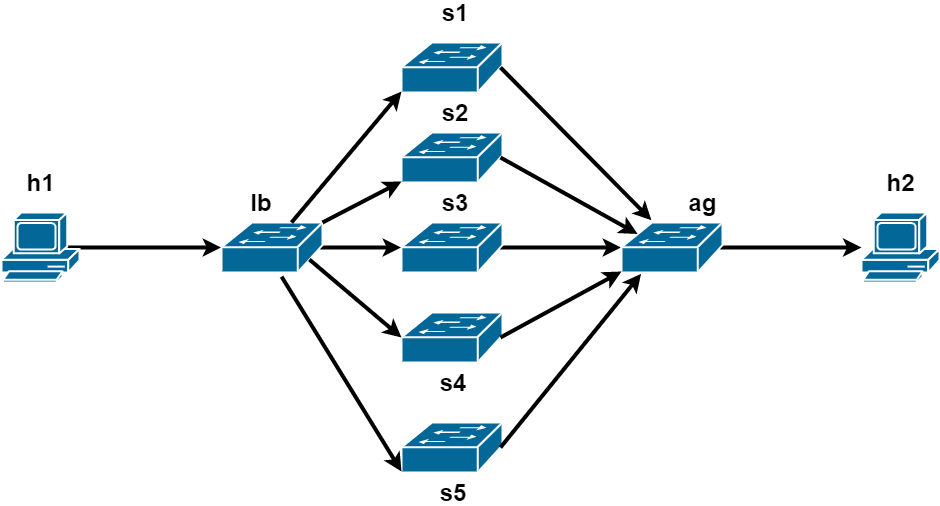
\includegraphics[width=1\textwidth]{figures/Herd_topology}
	\caption{Topology for the evaluation. h1 sends traffic over the loadbalancer, a Herd switch and the aggregating switch to h2.}
	\label{fig:topology_fig}
\end{figure}

As topology we use two host, $h1$ sends the traffic and $h2$ receives it. $h1$ sends to programmable switch $lb1$ which is there for load balancing. $lb1$ fowards the packets to the switches $s1 - 10$, which run the Herd protocol. The ingress switches $s1 - 10$ are an aggregating switch $ag1$ which is finally linked to the receiving host $h2$.\\

We had to separately build a load balancer for our test setup. In order to distribute the flows between the Herd switches the load balancing switch chooses randomly two Herd switches. The load balancer then forwards each packet of the flow to one of the two chosen switches. This has to be done this way since in the evaluation of the original paper each flow has exactly two switches observing each flow. Of course this procedure wouldn't be necessary in a real world application. There the number of observing switches would not be given by a separate switch, but according to the flows themselves, and therefore out of the direct control of the operators. Also the number of observing switches would not be limited by two. The coordinator would then forward this number to the switches according to the algorithm with the hello messages to take the locality of the flows into account.

Since the load balancing and the aggregating switch work differently from the ingress switch they get both their own controller and switch logic.

\subsubsection{Load-balancer}
The load-balancing switch chooses for each flow two random ingress switches and forwards the packets of that flow randomly to one of those two switches.
The corresponding controller forwards traffic to the ingress switches according to their switch ID.

\subsubsection{Aggregating switch}
The aggregating switch simply fowards every received to the end host.
Its controller receives the traffic from all ingress switches with Herd and forwards everything to the endhost.

\subsection{Traffic} \label{traffic}
To generate a sizeable amount of traffic on the sending host $h1$ we use CAIDA's anonymized Internet traces from 2016, like the original paper did. Using the $send.py$ script on $h1$ parses the packets stored in a $.pcap$ file and $h1$ forwards them through the testing topology. Further the script counts how often a packet was sent for each flow and writes flows that were seen more than $T$ times in $real\_elephants.json$ for later comparison with heavy-hitters found with Herd.

Configuring the parameters $\tau$, $r$ and $R$ in isolation might actually impact the accuracy of Herd negatively. Thus $tuningparameters.py$ simulates the whole protocol with given training data in order to reach the best possible accuracy for the running protocol.

However, since we had severe speed issues we weren't able to evaluate the protocol with five million packets like the original paper did. Using the whole five million packets would have taken around seven hours for each run. Since the evaluation also should have varying parameters this would have taken weeks for the assessment of each parameter, given that we have no errors. Thus we ended up using 100k and 400k packets, this takes two hours, respectively eight hours, with varying parameters.

%substitution for evaluation graphs and their discussion
\subsection{Evaluation} \label{evaluation}
\begin{figure}
	\centering
	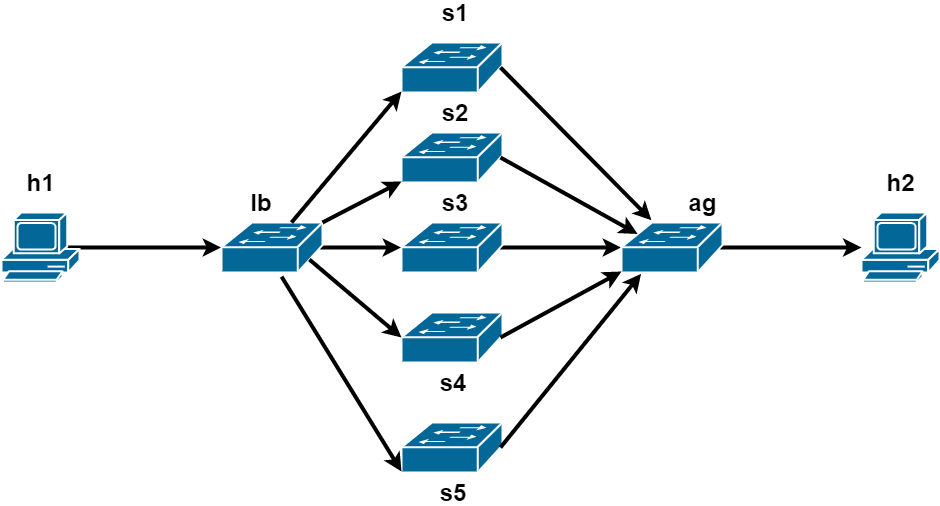
\includegraphics[width=0.5\textwidth]{figures/Herd_topology}
	\caption{some graph about the evaluation}
	\label{fig:topology_fig}
\end{figure}

\lipsum[1]
Something in %\figref{topology_fig}. %I still don't understand how \figrefs work.

\begin{figure}
	\centering
	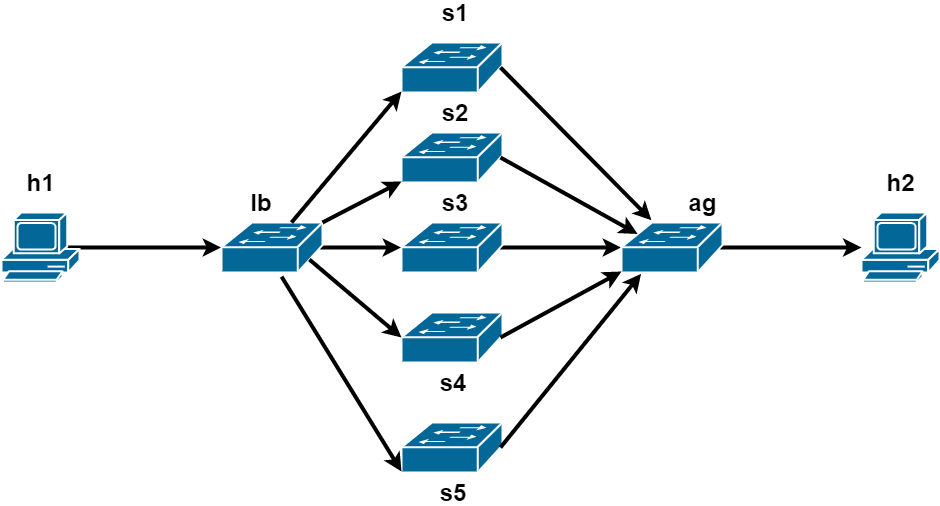
\includegraphics[width=0.5\textwidth]{figures/Herd_topology}
	\caption{some other graph}
	\label{fig:topology_fig}
\end{figure}
%\lipsum[1-2]

\section{Conclusion}
\hint{A brief conclusion about how you solved the project.} \\
We reimplemented Herd, a distributed heavy hitter protocol. Compared to the original paper we changed when to reset the flow/count tables. Further we had to implement a load balancing switch in front of the Herd switches for the evaluation. Additionaly, we had severe speed issues in the implementation in software compared to a implementation in hardware.

Further research could go towards improving the selection of the parameters. How it is implemented at the moment, the tuning has to be done offline, ahead of the protocol, with given training data. An improved protocol could maybe adjust the parameters according to captured data, and not prerecorded data. Even a dynamicaly changing tuning can be imagined which runs the tuning algorithm after certain events, e.g. after a timer or after reseting the hash tables. 

Another research topic would be, in case a single coordinator reaches its limit in processing power and speed, to have multiple coordinators, each responsible for a subnet, transferring data between each other.
%\lipsum[1]

\label{lastpage} % this must stay here
\clearpage
\addcontentsline{toc}{section}{References}
\bibliographystyle{acm}
\bibliography{refs}

\clearpage
\appendix
\pagenumbering{Roman}

\section{Group organization}
\hint{Briefly describe what each team member was contributing to the project}%still a bit lacking

\paragraph{Yannick Merkli}
%\lipsum[2]
\begin{itemize}
	\item coordinator
	\item controllers
\end{itemize}


\paragraph{Tim Bohren}
%\lipsum[3]
\begin{itemize}
	\item switch
	\item table values
	\item shell script for starting
\end{itemize}

\paragraph{Felix Rüssli}
%\lipsum[4]
\begin{itemize}
	\item tuningparameters
	\item realeleph to json
	\item report
	\item presentation
\end{itemize}

\end{document}
